\documentclass[letterpaper,twocolumn,10pt]{article}
\usepackage{url,epsfig,endnotes}
\providecommand{\keywords}[1]{\textbf{\textit{Keywords:}} #1}

\begin{document}

% Don't output date
\date{}

% Title
\title{\Large
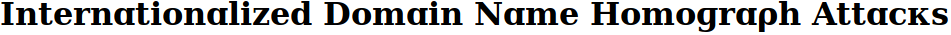
\includegraphics[height=\baselineskip]{title.png}
\\ \vspace{0.65mm} \large \normalfont
CSE 227: Computer Security - Spring 2017 \\ \textit{
University of California San Diego
}}

% Authors
\author{
{\rm Chen Lai\footnote{Author names are ordered lexicographically, by last name.}}\\
\normalfont{\texttt{chl588@ucsd.edu}}
\and
{\rm Zhongrong Jian\footnotemark[\value{footnote}]}\\
\normalfont{\texttt{zhjian@ucsd.edu}}
\and
{\rm J. Sidrach\footnotemark[\value{footnote}]}\\
\normalfont{\texttt{jsidrach@ucsd.edu}}
}

\maketitle

\abstract{
The invention of Unicode made it possible for non-English speaking people to enter the world of Internet. However, it also open up the possibilities of malicious use of URL. Sometimes different letters from different languages can look almost the same depending on the font. This paper mainly summarize the previous relevant work and analyze the current circumstance of Internationalized Domain Name Homograph Attack on the Internet via statistical approach on the websites from Alexa top 1 million rankings. Through the analysis results we will be able to provide some insight on this subject.
}

\keywords{Internationalized Domain Names, Homograph Attack, Phishing, Unicode, Punycode, Browser, Computer Security.}

\section{Introduction}
Domain names were originally designed to only support ASCII characters.
Internationalized Domain Names (IDNs) were proposed back in December 1996 by Martin D\"{u}rst\endnote{\url{https://tools.ietf.org/html/draft-duerst-dns-i18n-00}} for the purpose of letting non-English speaking people use Internet without additional restrictions.
This extension involves representing Unicode characters in ASCII using Punycode, so that they could be then rendered back into their Unicode representation.
Homograph letters (different letters whose representation is almost, if not, the same), however, present a potential security vulnerability.
For example, Cyrillic letter ``a'' can look identical to Latin letter ``a'' depending on the font.
In other languages, like Chinese, there exists many homograph letters between traditional Chinese and simplified Chinese.
Malicious attackers could then register a domain where one of the letters is actually Cyrillic but whose representation matched a Latin one.
Users could be linked to this newly registered malicious page, and they may not have any visual indication (at least without further interaction) that the page is not the one they think they are visiting.

In this paper, we analyze the potential impact of this type of attack, commonly referred to as IDN Homograph Attack.
Section 2 explains past and present policies of major browsers and top-level domain (TLD) registrants in an attempt to prevent the attack.
Section 3 explores relevant work in the literature related to homograph attacks.
Section 4 describes the methodology of data collection and analysis adopted in this project.
Section 5 comments the different results obtained.
Section 6 addresses the ethical concerns regarding the data collection.
Section 7 presents the conclusions obtained from this project.

\section{Background}
TODO
- Introduction to the section, two mayor players in preventing the attack, different roles: browsers vs TLDs

This section provides some background knowledge for mechanism that defends against internationalized domain name homograph attack.
There are two mayor players preventing the attack, the browsers and TLDs, with one working on the client side to detect and alert users while the other putting down policies on domain name registerar to restrict the number of possible homographs.

\subsection{Browsers}
TODO
- Rewrite, browser by browser: chrome, firefox, edge, safari
- Significant changes in the past years?
- Not updated browsers/embedded browsers?
- Screenshot of two actual domains that look the same but are different
- Cut screenshots better

Currently, most popular browsers will show the host name in Unicode depends on the language setting to defend IDN attack.
For example, Google Chrome\endnote{\url{https://www.google.com/chrome}} will display IDN in Unicode only if all characters of the domain names belong to only one language and this language has to be the user's preferred language. Figure \ref{screenshot} shows the screenshots of the original URL of \url{www.google.com} and its homograph.

\begin{figure}[t]
  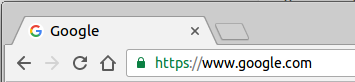
\includegraphics[width=\linewidth]{images/google}
  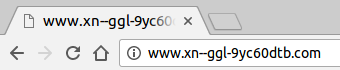
\includegraphics[width=\linewidth]{images/fakegoogle-punycode}
  \centering
  \caption{Google(top) and its homograph(bottom) on Chrome}
  \label{screenshot}
\end{figure}

The major browsers have their own IDN policies to defend against IDN homograph attack.
Google Chrome, starting with Chrome 51, will display Punycode if certain tests fail on the input URL.
These tests include but not limited to converting to Unicode, less than one numbering systems involved, no invisible characters, etc.

Internet Explorer\endnote{\url{https://support.microsoft.com/en-us/help/17621/internet-explorer-downloads}} displays URLs in IDN form if every component contains only characters from the languages configured in \textit{Internet Options}.

Firefox\endnote{\url{https://www.mozilla.org/en-US/firefox/new/}} uses a script mixing detection algorithm based on \textit{"Moderately Restrictive" profile of Unicode Technical Report 39} and displays Unicode when URL consists of any single script, any single script plus Latin, or it's in the white-list of other combinations.

Opera\endnote{\url{http://www.opera.com}} shows IDN only for whitelisted TLDs.

Safari\endnote{\url{https://www.apple.com/safari}} has a whitelist of scripts that do not contain confusable characters and only shows the IDN form for the whitelisted scripts.

\subsection{Top-Level Domains}
TODO
- What does different TLDs do
- ccTLDs

The Internet Corporation for Assigned Names and Numbers(ICANN) is an organization responsible for the management of domain name system. In 2009, ICANN started to accept the application for internationalized country code top-level domain(IDN ccTLD) for the benefits of non-English speaking people and the first IDN ccTLD was added to DNS root zone in 2010\ref{tld1}.

ICANN is aware of the potential vulnerability of homograph attacks and limits the usage of letter that is similar to Latin. For any application of potential IDN ccTLD, if there exists letter that is similar to an existing TLD, ICANN may reject them, especially for two-letter TLD. Three-letter TLD have higher chance to be accepted, as they are considered to be safer than two-letter TLD. ICANN listed detailed checking process in the Final Implementation Plan\ref{icann}.

Although the vulnerability of homograph has been introduced as early as 2001, most registrant of TLD don't have the policy to defend homograph attack. Only several TLD have published policy to eliminate the potential risk of specific language. For example, .cn .biz, .hk, and all Chinese TLD will activate both traditional Chinese domain and simplified Chinese domain once one of it is registered. Registering with characters in both traditional Chinese and simplified Chinese is not allowed.

- TODO it was found in wiki, but i didn't find source document.
(In .org domain, once one letter is used in the domain, other homograph letters corresponding to the same domain will be prohibited.)

For the second level domains, some registrant registers similar IDNs for brand protection, like Google. Google has registered most IDN in 2005.

\section{Related Work}
Several relevant studies have been conducted to describe the potential security issues with internationalized domain names, while providing possible solutions to mitigate the surface attack of these homograph domain names. The first of these studies, \textit{The Homograph Attack}~\cite{gabrilovich2002}, was written by Evgeniy Gabrilovich and Alex Gontmakher in 2001, and proved the feasability of the attack.

In 2006, Vicktor Krammer proposed a defense mechanism based on address bar highlighting on the browsers and a better user interface~\cite{krammer2006}.
This method of defense mainly targets regular users, by making them explicitly aware of the URL differences.
It checks each character in a URL separately, highlighting digits or characters of various scripts in different background colors, so that users can easily tell the difference.
It also suggests using larger font sizes in the address bar, to help distinguish possible homograph characters from their Latin counterparts.

In 2012, Maurer and H\"{o}fer argued that safe-guards based on browsers' blacklists was far from enough to protect users from sophisticated phishing attacks~\cite{maurer2012}.
They proposed a more complex method based on URL components and the spell checking functionality of any search engine.
In this method, a URL is be divided into several parts, namely, base name (the primary domain name as registered at the registrar), sub-domain (part before the primary domain, i.e., before the last identifier and TLD), path domain (sub-folder of the URL), and brand name (any popular brand name that is present in the URL).
Their algorithm tries to prevent the attack by analyzing each of these URL parts.
Each one is sent to the search engine for a spelling check, and in the cases that a spelling suggestion is returned, the URL will be marked as suspicious.
By splitting the URL into these parts, this method aims to cover almost all possible cases of confusable URLs or domain names.
However, this mechanism relies exclusively on the search engine to return spelling suggestions, and as a result, it is highly dependent on the search engine and query itself.

While these last two methods were not adopted, they have influenced other possible mitigations currently implemented in most modern browsers.
For instance, the base name of the URL is displayed in a darker color in Google Chrome and Mozilla Firefox.
Safari goes a step further and only shows the base name of the URL.

Other attempts to analyze the impact of homograph attacks have also been made.
In 2009, Peter Hanay and Christopher Bolan~\cite{hannay2009} concluded that, while most modern browsers in fact have implemented useful measures to prevent internationalized domain name homograph attacks, email clients where not nearly as effective, specially when dealing with incoming emails.
In 2010, Johnny Al Helou and Scott Tilley~\cite{al2010} argued that the introduction of country-code Top Level Domains (ccTLDs) have made this attack easier to perform again.

Our approach to analyze the potential security risk of homograph internationalized domain names was fundamentally different the ones evaluated.
Rather than inspecting traffic or generating random homograph permutations of a string, we took a more systematic approach.
We clustered all internationalized homograph domains using a snapshot of the \texttt{.com} domain zone.
We then used a list of top web sites and domain registrants data to classify each homograph domain name.

\section{Methodology}
Our data collection involved two primary sources.
The first one was a snapshot of the \texttt{.com} and \texttt{.net} domain zone, from now on referenced as \textit{.com snapshot}.
This snapshot was provided by Verisign\endnote{\url{https://www.verisign.com/en_US/channel-resources/domain-registry-products/zone-file/index.xhtml}}, and it is dated on 2017/05/01.
It contains, for the most part, the name servers of all \texttt{.com} and \texttt{.net} domains.
For the purposes of this project, only the \texttt{.com} domains were considered.

The second data source was the \textit{Alexa Top 1 million sites ranking}\endnote{\url{https://www.alexa.com/topsites}}, from now on referenced as \textit{top domains snapshot}.
It contains the most popular one million web sites (as ranked by Alexa), regardless whether they are \texttt{.com} domains or not.
It was also retrieved on 2017/05/01.

In an effort to help with the reproducibility and replicability of this project, the original data and processing code used in this project has been made available in a public repository\endnote{\url{https://github.com/jsidrach/idn-homograph-attack}}.

\subsection{Data Processing}
We used the \textit{.com snapshot} to obtain all the internationalized domains of the \texttt{.com} domain zone.
All internationalized domain names are represented using Punycode, so they start with the \texttt{xn--} prefix.
Using this information we first filtered the \textit{.com snapshot} to match only the \texttt{.com} domains that start with \texttt{xn--}.
Since the \textit{.com snapshot} contains name server records, a single domain may have more than one entry in the file.
Only the domain name is relevant for this project, so the rest of the columns of the \textit{.com snapshot} were discarded.
We sorted the domains in lexicographical order, removing duplicates in the process.

We used the \textit{top domains snapshot} as a source for the canonical (non-international) domain name of a website, based on its ranking.
As we were only interested in non-internationalized domain names, we discarded the ones that start with the prefix \texttt{xn--}.
We also removed sub-domains, since we only had top-level domain names in the \textit{.com snapshot}.

\subsection{Clustering}
The underlying assumptions behind the clustering process are that homograph attacks are more likely to target popular domains, and that the million domains from the \textit{top domains snapshot} contains most of the popular domains.
To detect potential internationalized domain name homograph attacks, we clustered the internationalized domain names in the \textit{.com snapshot}.
The representative of each cluster is a homograph domain name from the \textit{top domains snapshot}, which we called canonical domain name.
Only clusters with at least one internationalized homograph domain name were output.

The detection of homograph domain names was done using an algorithm to check if two strings are confusable.
This algorithm is described in the \textit{Unicode Technical Standard \#39}\endnote{\url{http://www.unicode.org/reports/tr39}}.
The approach followed has some caveats, that could be addressed in future work.
For instance, it does not detect a homograph of \texttt{www.google.com}, where the first ``.'' has been replaced by a similar looking Unicode character.
More sophisticated homographs can also be generated by using Unicode characters similar to ``/''.
It is also worth noting that only domain names from the \texttt{.com} zone were considered, but similar studies could be done to other top-level domains following the same procedure.
All things considered, we still think this approach is a valuable first step.

Another type of clustering was also performed.
We grouped the homograph domain names by its registrant organization, and ranked each organization by the number of homograph domain names to their name.
This could shed light on which registrant organizations are allowing homograph domain names, or even on which individuals and companies are doing it the most.

\subsection{Manual Classification}
The last part of the data processing was the classification of the homograph domain names.
This classification was done manually, to be able to differentiate between scam and unrelated websites.
To help with the classification and speed up the process, we queried the \textit{WHOIS} records\endnote{\url{https://whois.icann.org}} of every homograph domain name.
Some domains had expired at the time of the classification, and were subsequently deleted from the output file.

The two high level categories that were defined are \textit{Canonical} and \textit{Third Party}.
The first one, \textit{Canonical}, was employed when the domain is registered by the same organization as its canonical homograph domain name.
The second one, \textit{Third Party}, was used when the domain is registered by a different organization than its canonical homograph domain name.
Additionally, a more detailed classification was made:
\itemize{
\setlength{\itemsep}{0pt}
\setlength{\parskip}{0pt}
\setlength{\parsep}{0pt}
\item \textit{Canonical - Parking}: domain was registered but it was not accessible via HTTP.
\item \textit{Canonical - Redirect}: domain redirected (HTTP Status Code 301/307/308) to its canonical homograph domain name.
\item \textit{Third Party - Redirect to Canonical:} domain redirected (HTTP Status Code 301/307/308) to its canonical homograph domain name.
\item \textit{Third Party - Unrelated}: domain resolved, but the contents of the website were totally unrelated to its canonical homograph domain name.
\item \textit{Third Party - Parking}: domain was registered, but it was not accessible via HTTP, or when accessed, a default domain parking web page was displayed.
\item \textit{Third Party - Scam}: domain resolved, and the website displayed was a clear attempt (similar color, logos, etc.) to make users think they were visiting the canonical homograph domain name.
}

\section{Results}

\begin{table*}[ht!]
\centering
\begin{tabular}{lrr}
\hline
Domains                                           & \#                         & \%                         \\ \hline
\itshape\sffamily{Canonical domain names}         & \itshape\sffamily{458731}  & \itshape\sffamily{8.31\%}  \\
\hspace{0.5cm} With IDN homographs                & 825                        & 6.04\%                     \\
\hspace{0.5cm} Without IDN homographs             & 457906                     & 2.27\%                     \\
\itshape\sffamily{Internationalized Domain Names} & \itshape\sffamily{1045400} & \itshape\sffamily{91.69\%} \\
\hspace{0.5cm} With canonical homograph           & 1099                       & 3.68\%                     \\
\hspace{0.5cm} Without canonical homograph        & 1044301                    & 2.74\%                     \\ \hline
\end{tabular}
\caption{Overview of the clustering results.}
\label{clustering-results}
\end{table*}

We obtained 458731 domain names from the \textit{top domains snapshot} that belonged to the \texttt{.com} zone.
From the \textit{.com snapshot}, we identified a total of 1044301 internationalized domains.
However, only a low percentage of the internationalized domain names (3.68\%) had a matching homograph canonical domain name in the \textit{top domains snapshot}.
Even if we take into account that our homograph detection algorithm is rather limited (as described before), these results still indicate that the majority of internationalized domain names are not being used in homograph attacks.
An overview of these clustering results can be found in Table~\ref{clustering-results}.

Table~\ref{top-com-alexa-with-idns} shows the number of internationalized domain name homographs for the top ten \texttt{.com} domains.
It is worth noting that most of the homograph domains of \textit{google.com} are actually registered by Google, possibly as a defensive measure.
Another surprising result of the homograph clustering is that 81.87\% of the groups have just one homograph internationalized domain name.
This suggests that this kind of attack may not be targeted only to top websites, but rather to any domain where valuable information could be obtained from the users by a scam.

\begin{table}[ht!]
\centering
\begin{tabular}{lr}
\hline
Domain       & \# of IDN homographs \\ \hline
google.com   & 24                   \\
youtube.com  & 3                    \\
facebook.com & 9                    \\
baidu.com    & 3                    \\
yahoo.com    & 4                    \\
reddit.com   & 1                    \\
qq.com       & 2                    \\
taobao.com   & 1                    \\
live.com     & 1                    \\
vk.com       & 6                    \\ \hline
\end{tabular}
\caption{Top ten .com domains in the Alexa ranking with IDN homographs.}
\label{top-com-alexa-with-idns}
\end{table}

The manual classification sheds some light on how these homograph internationalized domain names are currently being used.
For the most part (82.34\%), the domains are registered by a third party, and not being used actively (parking).
One possible explanation for this is that the domain was bought in an attempt to be re-sold later at a higher price to the owner of the matching canonical homograph domain.
However, the potential security risk is still present as there are no guarantees that the parked domains will remain inactive in the future.
A detailed breakdown of this classification can be found in Table~\ref{manually-classified-idns}.

\begin{table}[ht!]
\centering
\begin{tabular}{lrr}
\hline
Status                               & \#                     & \%                         \\ \hline
\itshape\sffamily{Canonical}         & \itshape\sffamily{88}  & \itshape\sffamily{8.31\%}  \\
\hspace{0.5cm} Parking               & 64                     & 6.04\%                     \\
\hspace{0.5cm} Redirect              & 24                     & 2.27\%                     \\
\itshape\sffamily{Third Party}       & \itshape\sffamily{971} & \itshape\sffamily{91.69\%} \\
\hspace{0.5cm} Redirect to Canonical & 39                     & 3.68\%                     \\
\hspace{0.5cm} Unrelated             & 29                     & 2.74\%                     \\
\hspace{0.5cm} Parking               & 872                    & 82.34\%                    \\
\hspace{0.5cm} Scam                  & 31                     & 2.93\%                     \\ \hline
\end{tabular}
\caption{Breakdown of the manually classified homograph IDNs.}
\label{manually-classified-idns}
\end{table}

Table~\ref{top-registrants-homograph-idns} contains the top ten registrants with the most homograph internationalized domain names.
Most of these registrants are actually domain privacy companies, so it is impossible to know if the domains belong to the same person or not.
There are also several individuals with a high number of homograph internationalized domain names.
It is also worth mentioning that some of these individuals seem to be targeting specific industries.
For instance, a single person has registered homographs of ``audi'', ``citroen'' and ``diesel''.

\begin{table*}[ht!]
\centering
\begin{tabular}{llr}
\hline
Registrant organization              & Registrant email           & \# of homograph IDNs \\ \hline
Domains By Proxy, LLC                & --                         & 89                   \\
Super Privacy Service c/o Dynadot    & privacy@dynadot.com        & 23                   \\
Domain Registries Foundation         & --                         & 22                   \\
Duong Thien                          & thiendv@outlook.com        & 18                   \\
Syngenuity Limited                   & manager@syngenuity.com     & 12                   \\
Helpnet: Brand Development \& Sales  & help@strongestbrands.com   & 12                   \\
ONUNO L.L.C.                         & corucas@gmail.com          & 11                   \\
Privacy Protection Service INC d/b/a & contact@privacyprotect.org & 10                   \\
Hubertus Henz                        & hu\_h5@yahoo.de            & 9                    \\
wuyu                                 & wy65535@126.com            & 7                    \\ \hline
\end{tabular}
\caption{Top ten registrants with the most homograph IDNs.}
\label{top-registrants-homograph-idns}
\end{table*}

\section{Ethical Considerations}
The domain information used in this project is publicly available, and was voluntarily provided by the registrants of the domains when they registered them.
The full \texttt{.com} domain zone snapshot will not be publicly disclosed, as its access requires a paid subscription.
The retrieval of the \textit{WHOIS} information was performed only for the homograph internationalized domain names, which were about one thousand.
It was performed with a significant delay between petitions (3 seconds) in order to avoid saturating the servers.

\section{Conclusions}
TODO
- Conclusions of our work
- Possible future work
- TLDs
- Hard to balance (rendering idn useless vs preventing the attack)

\section*{Acknowledgments}
We would like to thank Louis DeKoven and Stefan Savage for their help and support throughout this project.

{\footnotesize \bibliographystyle{acm}
\bibliography{bibliography}}

\theendnotes

\end{document}
